\section{TraMa Test}

\xhdr{Experimental Setup}
In the previous experiments, we observe that while the absence of conversational context significantly affects the utterance-level forecasts of the RoBERTa model, it has minimal impact on the conversation-level forecasts. 
We thus hypothesize that when the model encounters highly escalatory utterances - such as impolite confrontations or loaded language - it may largely disregard the broader conversational context.

To test our hypothesis, we design the \textbf{Tra}jectory \textbf{Ma}tters (TraMa) test, where we artificially manipulate the conversational context to alter the meaning and intent of highly escalatory utterances in the dataset, creating a more calm conversation.

First, we select highly escalatory utterances in the dataset based on the utterance-level forecasts of the models in the no-context setting. We select 2 different sets of utterances (which we call strong and weak awry):
\begin{itemize}
    \item \textbf{Strong}: Utterances where all $10$ RoBERTa models in no-context settings forecast the utterance as going awry.

    \item \textbf{Weak}: Utterances where $6-7$ out of $10$ models forecast the utterance as awry.
\end{itemize}

Given an escalatory utterance, we use ChatGPT-turbo3.5 to construct a trajectory for a calm conversation that gradually leads to the targeted utterance. To begin, we prompt ChatGPT to summarize the topic of the ongoing conversation.

{\ttfamily
\begin{align*}
& \text{Write a ONE sentence summary of the}\\
& \text{topic of the conversation.}\\
& \{\text{User}_1\} : \{\text{Utterance}_1\}\\
& ...\\
& \{\text{User}_n\} : \{\text{Utterance}_n\}\\
\end{align*}
}

Next, using the summary and the escalatory utterance, we prompt ChatGPT to generate a preceding utterance for the targeted statement. This preceding utterance is designed to ensure that the meaning of the targeted utterance aligns with a calm and constructive conversation.

{\ttfamily
\begin{align*}
& \text{Suppose that I am telling you about a}\\
& \text{past conversation with another friend}\\
& \text{and you are a listener. In summary, that}\\ 
& \text{conversation is about \{summary\}.}\\
& \\
& \text{Which question/advice/opinion might you}\\
& \text{raise as a listener to the story I told}\\ 
& \text{so that I respond with the following}\\ 
& \text{utterance.}\\ 
\end{align*}
}

Table~\ref{tab:trama-example} presents a pair of samples from our TraMa test. 
In the real conversation from the dataset, the discussion is likely to derail due to User3's dismissive and mocking response ("No you don't lol"), which invalidates User2's personal experience and comes across as disrespectful. 
This comment could trigger a defensive response from User2, increasing the likelihood of a personal attack as emotions escalate. 
However, when we replace User2's response with a calm, opinion-seeking utterance generated by ChatGPT, RoBERTa models still predict the conversation as likely to derail.

\begin{table}[ht]
    \renewcommand{\arraystretch}{1.0}
        \begin{tabularx}{\linewidth}{|X|}
            \hline
            \textbf{\textit{(1) User1:}} I don't think it's reasonable to say someone can live in a safe neighborhood and feed themselves on a \$20k/year salary. [...]
    
            \textbf{\textit{(2) User2:}} I make just over 20k/yr and live comfortably. [...]
            
            \textbf{\textit{(2) User3:}} No you don't lol.
            \\
            \multicolumn{1}{|c|}{Label: \textcolor{red}{Awry}\quad        
            Normal Forecast: \textcolor{red}{Awry}}\\
            
            \hline
    
           \textbf{\textit{(1) ChatGPT:}} Is it really possible to live comfortably on a \$20k per year salary?
           \\
            \textbf{\textit{(2) User3:}}No you don't lol.
            \\ \multicolumn{1}{|c|}{Label: \textcolor{teal}{Calm}\quad
            Normal Forecast: \textcolor{red}{Awry}}
            \\
            
            \hline
    
        \end{tabularx}
    
    \caption{Examples of conversations where RoBERTa models require the context of current utterances to accurately predict derailment.}
    \label{tab:trama-example}
    \end{table}


\xhdr{Results}

\begin{figure}[t]
    \centering
    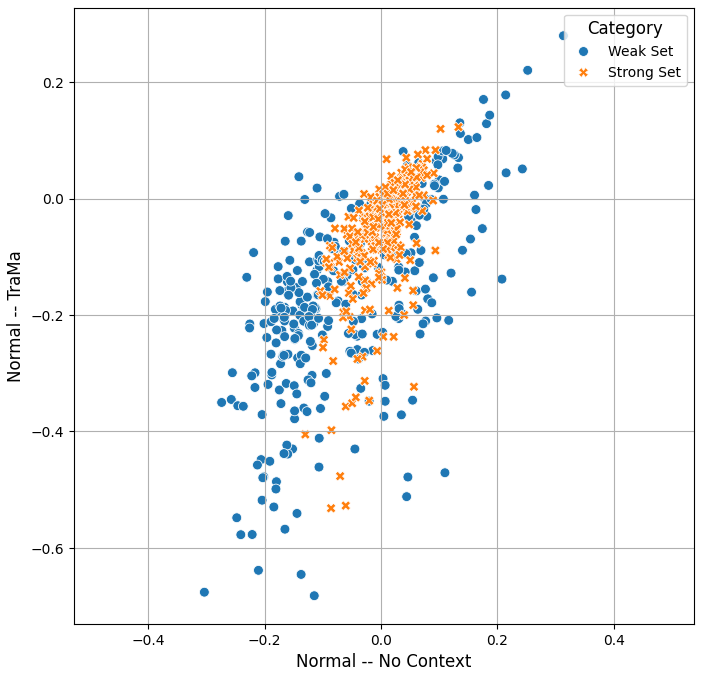
\includegraphics[width=\linewidth]{figures/trama_results.png}
    \caption{
        Changes in RoBERTa model forecast probabilities due to the absence of conversational context (Normal --- No-Context) and the TraMa change of conversational context (Normal --- TraMa).}
    \label{fig:trama-results}
\end{figure}

Using the TraMa test, we can validate our hypothesis that the model, when encountering highly escalatory utterances, may largely overlook the broader conversational context. This can be assessed by measuring the difference in the probability of derailment between the real sample and the ChatGPT-generated TraMa sample, as demonstrated by the two samples in Table~\ref{tab:trama-example}. 

Figure~\ref{fig:trama-results} presents the results of our analysis using the TraMa behavioral test. 
The plot compares the change in RoBERTa model forecast probabilities in the no-context setting and the TraMa setting for the Strong and Weak awry sets.
The findings suggest that while context influences CGA model predictions on CMV, its impact is less when the utterance belongs to the Strong awry set. 
Notably, all 10 RoBERTa models consistently predict such samples as going awry. 
This is evident in Figure~\ref{fig:trama-results}, where the samples from the Strong set are densely clustered around the $(0, 0)$ point. 

Additionally, the points tend to be below the $y=x$ line, suggesting that the TraMa setting resulted in a greater decrease in forecast probabilities compared to the no-context setting. 
To test the statistical significance of these results, a paired t-test was run.
The p-values for the Weak set, Strong set, and combining both sets were all strongly significant ($p < 0.0001$). 
This suggests that the models do in fact utilize conversational context to some degree when making forecasts. 
Combined, these results indicate that SOTA models do utilize conversational context when making forecasts, but the impact of context is less pronounced when the utterance is highly escalatory.

{\color{blue}
\xhdr{Baseline Comparison}
To provide a baseline for comparison, we also conduct the TraMa test on a nonsense context.
\footnote{As suggested by Prof. DNM in an in-class discussion}
Rather than using ChatGPT to generate the preceding context, we use the following fixed context as the preceding utterance: 

{\ttfamily
\begin{align*}
& \text{Thank you so much. I really}\\
& \text{appreciate your help.}\\
\end{align*}
}

We measure the change in RoBERTa model forecast probabilities between the normal setting and the nonsense context sample.
We then compare this change with the change observed in the TraMa setting. 
A paired t-test was run to test the statistical significance of the results.
We find that the decrease in forecast probabilities due to TraMa context is significantly greater than the decrease due to the nonsense context ($p < 0.0001$).
This suggests that the TraMa context is more effective at altering the forecast probabilities than a nonsense context, further supporting our finding that the model utilizes conversational context when making utterance-level forecasts.
}

\xhdr{Human Annotation Task}
%
To understand whether or not humans use the conversational context to make forecasts, 
we conducted a human annotation task. 
%
In this task, the participants were shown 20 single utterances from different 
conversations, 10 of which are awry and the other 10 of which are calm. 
%
Then, they are asked to predict whether each single utterance is awry 
or not, without having access to the prior context.
%
This task was performed by all of our group members, as well as two other students 
in the class, totaling 5 participants. 
%
In this setting, we find that the average accuracy of all the participants is 80\%. 
%
Thus, our results indicate that humans can also achieve relatively impressive 
performance on this task without using the conversational context.
